\chapter{Produktprincip}
Produktets vil være en webapp løsning, som ved brug af Googles bruger API og fragtfirma 
api'er såsom GLS's og Postnords API'er. skal kunne gennemsøge den brugerens gmail og 
derudfra hente trackingnummer på forsendelser fra en bred vifte af fragtfirmaer. denne 
tracking information skal derefter fremvises til brugeren på webappen, således tracking 
informationen fra alle brugerens pakker samles.
\section{Flowchart over programmet}
\begin{figure}[h]
    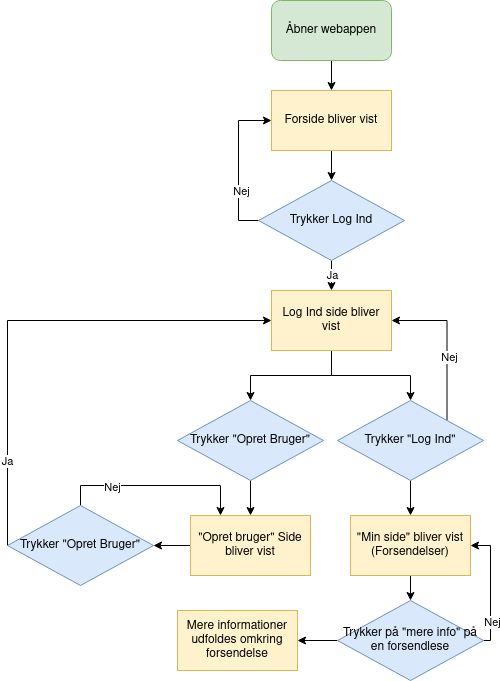
\includegraphics[width=0.5\linewidth]{Pictures/flowchat-main.png}
    \centering
    \caption{General funktion af programmet.}
     \label{fig:Flowchat}
  \end{figure}
  

\section{Produktkrav}
Der er her opstillet en række hårde og bløde krav som det udviklede web app skal opnå. de er som følger:

\subsubsection{Hårde krav}
\begin{itemize}
    \item Skal kunne tracke pakker fra mindst 2 forskellige fragtfirmaer
    \item Skal kunne fremvise pakke tracking fra mindst 2 forskellige fragtfirmaer det samme sted
    Oprette bruger
    \item siden skal have en lav kompleksitet (tilgå tracking på 2 klik)
\end{itemize}

\subsubsection{Bløde krav}
\begin{itemize}
    \item Skal have et moderne stilrent design
    \item Oprette bruger med Google
    \item Skal fungere upåklageligt på mobile enheder (være responsivt)
    \item Skal selv kunne hente mails fra brugerens google konto
\end{itemize}
\section{Tech-stack}
Webapplikationens tech stack består af Html hvor vi bruger razorpages og til styling bruges css her bruger vi Tailwind som er et
css framework. Der bruges også javascript og her bruger vi også javascript bibliotekket jQuery som har til formål
at programmere webapplikationer. Til backend bruges Csharp og som database bruges mssql.
\section{Database}
Til Databasen bruges MS SQL som er en relations database(RDBMS) udviklet af Microsoft. Hvilket
giver mest mening når man laver Asp.net core mvc webapps da mange dele af dette bygger på at man bruger
MS SQL. Til kommunikation mellem MS SQL og Asp.net core 7 mvc projektet.    

Til at lave migrations til databasen bruges Entity Framework Core .NET Command-line tools. 
Hvorman så kan skrive Models i projektet og putte dem ind i vore Application database 
context. Her brugesto kommando'er første kommando laver en migration fra ApplicationDbContext.cs 
som er den databasecontext til vores database hvor der opbevares data om brugeren der skal gemmes. 
Den næste kommando opdateres så databasen med migration som vi lavede før. Af sikkerheds grunde er der 
valgt at databasen er delt i to en hvor alt login data blivver gemt og en hvor data om bruger bliver gemt.
Det gør at hvis der bliver udført et sql angreb er det kun den en af databaserne der bliver ramt.

\begin{figure}[!h]
    \begin{lstlisting}[language=bash]
        > dotnet ef migrations add IntialUserData --context ApplicationDbContext
        > dotnet ef migrations add IntialUserLogin --context IdentityDbContext
        > dotnet database update --context ApplicationDbContext
        > dotnet database update --context IdentityDbContext
    \end{lstlisting}
\end{figure}

\begin{wrapfigure}{r}{0.5\textwidth} 
    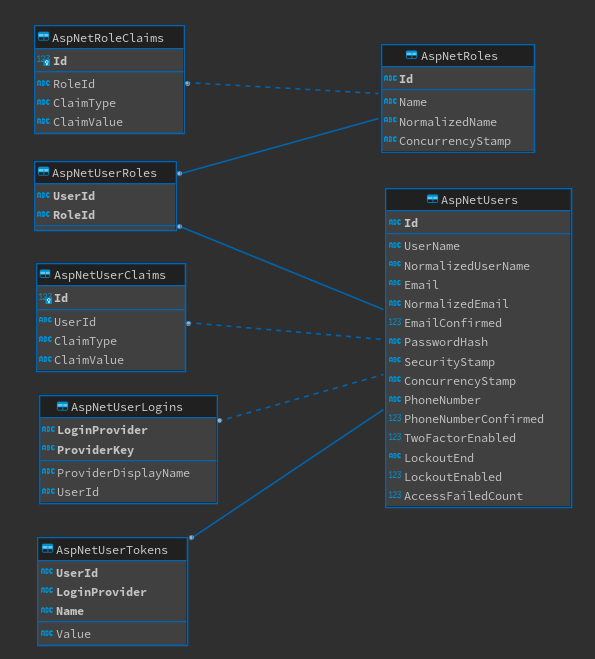
\includegraphics[width=0.4\textwidth]{./Pictures/database-diagram.png}
    \caption{Uklip af User tablen i Databasen}
    \label{fig:databaseUserTable}
\end{wrapfigure}

På figur 4.2 kan man se den overordnet database struktur. Denne database er lavet med
Asp.net core Identity som er en API som giver nogle login funktionaliteter til ens program
og kan findes som en nuget package. Denne Api genere selv modellerene til systemet.  




\section{Asp.net Identity}
Asp.net core er det som bliver brugt til håndtere autentificering og autorisation i webapplikationen.
Denne måde at gører det på giver en standardiseret måde at håndtere dette på. Identity giver også indbygget
funktionaliteter til at håndtere brugerregistrering, login, håndtering af adgangskoder og meget mere.

\subsection{Google OAuth}
Google OAuth bruger OAuth som er en åben protokol som alle kan bruge. Denne protokol bygger på
HTTP protokolen. Ved hjælp at OAuth kan man som tredjepartsapplikation få adgang til brugers data.
Det er det vi skal brgue den data vi godt vil have fandt i fra brugeren er at læse brugers emails. 
Til at få emails fra Google bruges Googles gmail API. som gør det muligt at læse alle brugers emails når de
er logget ind med OAuth.
\newpage
\section{Wireframes}

\begin{wrapfigure}{r}{0.3\textwidth} 
    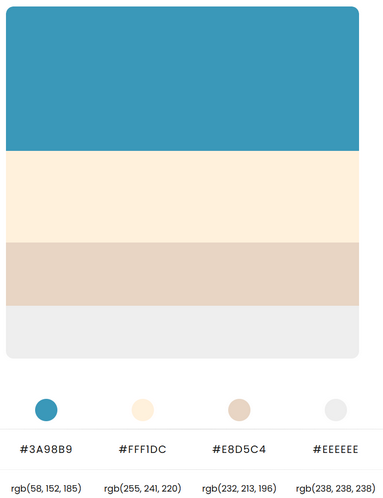
\includegraphics[width=0.3\textwidth]{./Pictures/Colorpallete.png}
    \caption{Colorpallete der er brugt.}
    \label{fig:Colorpallete}
\end{wrapfigure}

som man kan se på figur 4.3 har vi forsiden. Her er der en navbar. Hvor man kan vælge nogle muligheder. man
kan gå til om os som er en side der fortæller noget om virksomheden. så kan gå til login hvor man også kan registere sig.
hvis man også trykker på start vil man blive ført til registering. Farve valget er ikke tilfældeligt vi bruger den samme farve
palette igenmen hele webapplikationen. 

\begin{wrapfigure}{r}{0.5\textwidth} 
    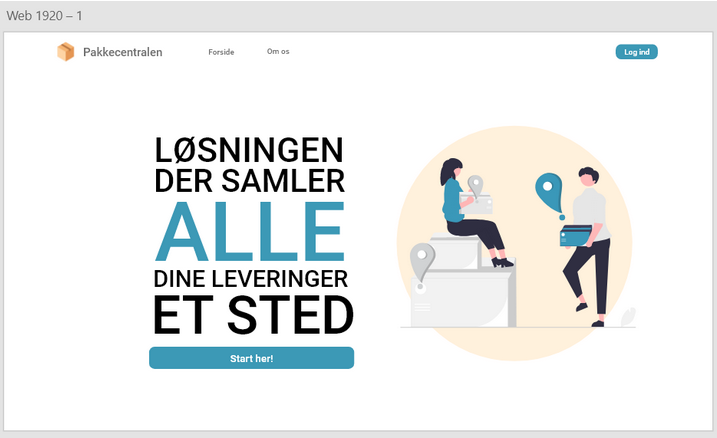
\includegraphics[width=0.5\textwidth]{Pictures/Wireframe1.png}
    \caption{Wireframe af førsiden af webapplikationen}
     \label{fig:Wireframe1}
  \end{wrapfigure}

  

  \begin{wrapfigure}{r}{0.5\textwidth} 
    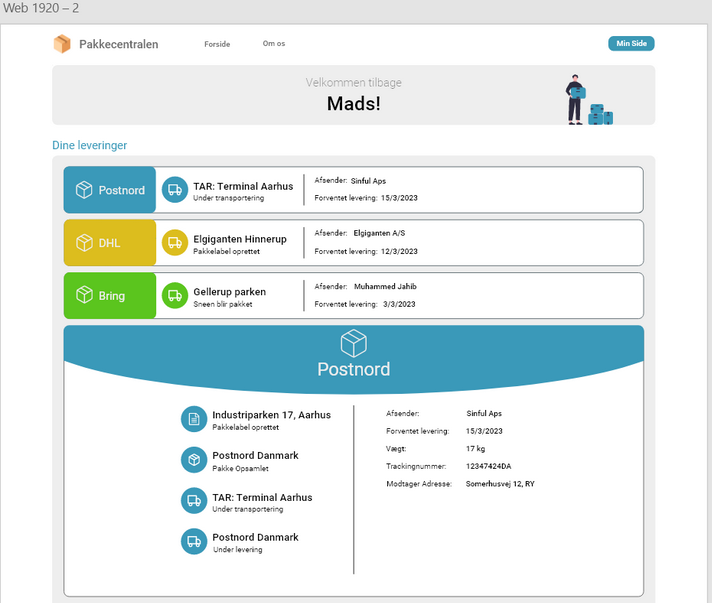
\includegraphics[width=0.5\textwidth]{Pictures/Wireframe2.png}
    \caption{Wireframe af hvor man kan se sin}
     \label{fig:Wireframe2}
  \end{wrapfigure}